\section{Design and Implementation}
\label{sec:implementation}

\subsection{Radix Tree}

DM-Cache currently employs a hash table for managing the cached blocks. Eviction
of cached blocks is done when there is a conflict in the hash table where two
blocks map to the same entry. Cache sizes are also restricted to powers of two
in size because of the hash function used in the implementation.

In order to improve cache management and remove the cache size restrictions the
hash table was replaced with a radix tree. This allowed for implementation of
the LRU (Least Recently Used) and LFU (Least Frequently Used) cache management
algorithms.

\subsection{Dynamic Disk Spin}

\begin{figure}[t]
  \caption{Client Server Daemon Communication Architecture}
  \centering 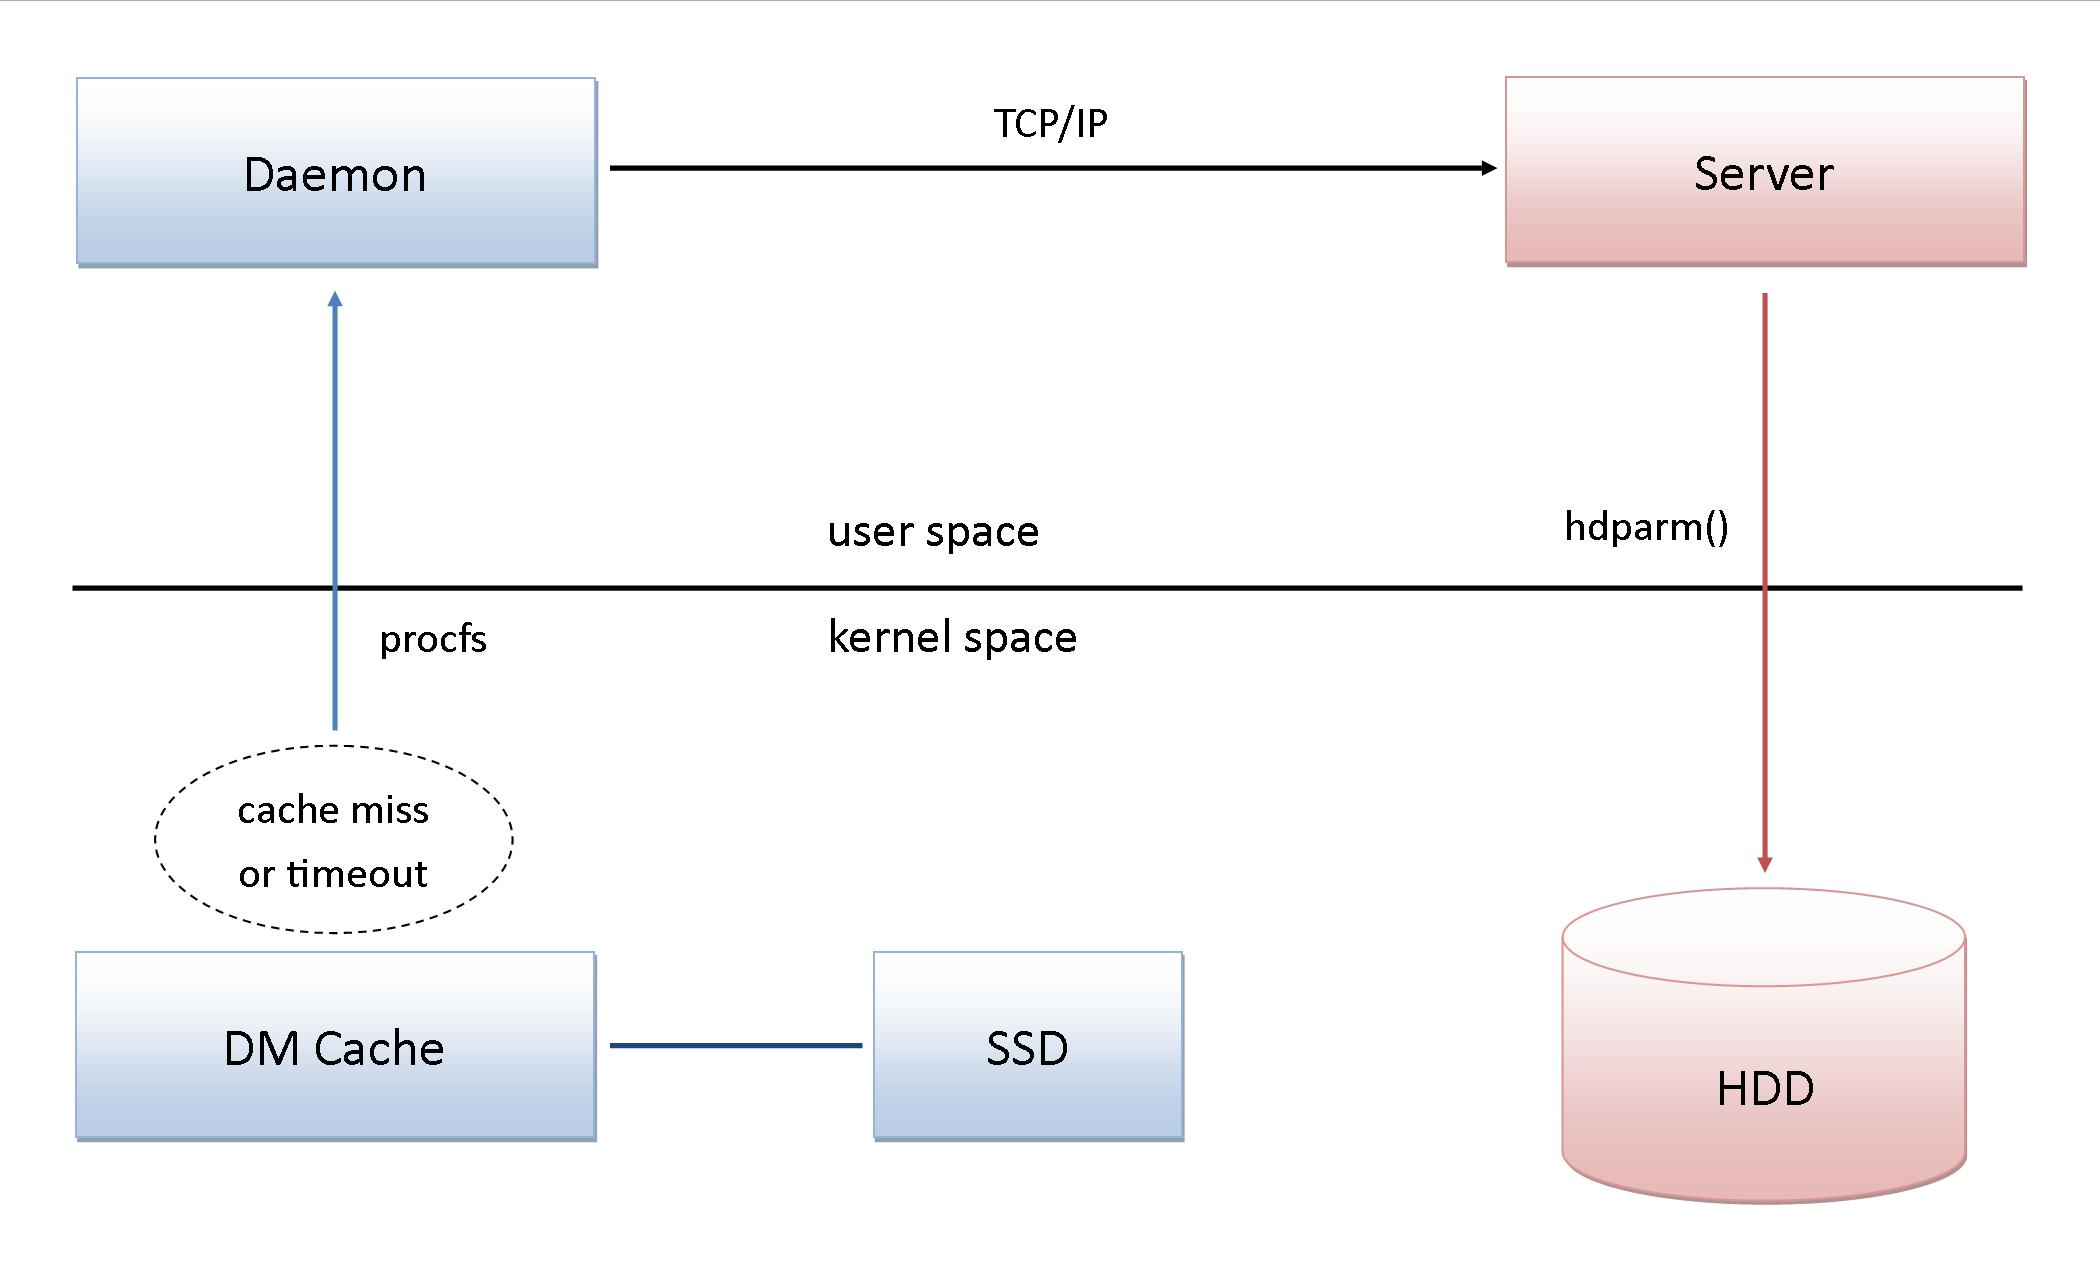
\includegraphics[width=\linewidth]{daemon.png}
  \label{fig:daemon}
\end{figure}

In our implementation, we use a user space daemon that interacts with the
storage server for dynamically spinning the disk up or down. The setup for the
spinning mechanism includes the user space client daemon, a web server that
listens for incoming disk commands, and a kernel thread that checks the time
since the last cache miss, notifying the client daemon when it is time to spin
the disk down.

After a cache miss, if the disk is not spinning, DM-Cache will block until the
client daemon successfully sends a spin up request to the storage server and the
storage server responds with an acknowledgment, confirming that the disk is
spinning. The mechanism for communication between user space and kernel space is
an in-memory data structure that is exported as a Linux proc file system file
for access by user applications. Both our modified DM-Cache module and the
client daemon will read from and write to this file.
